\begin{center}
  \Large
  \textbf{BIOGRAFI PENULIS}
\end{center}

\addcontentsline{toc}{chapter}{BIOGRAFI PENULIS}

\vspace{2ex}

\begin{wrapfigure}{L}{0.3\textwidth}
  \centering
  \vspace{-3ex}
  % Ubah file gambar berikut dengan file foto dari mahasiswa
  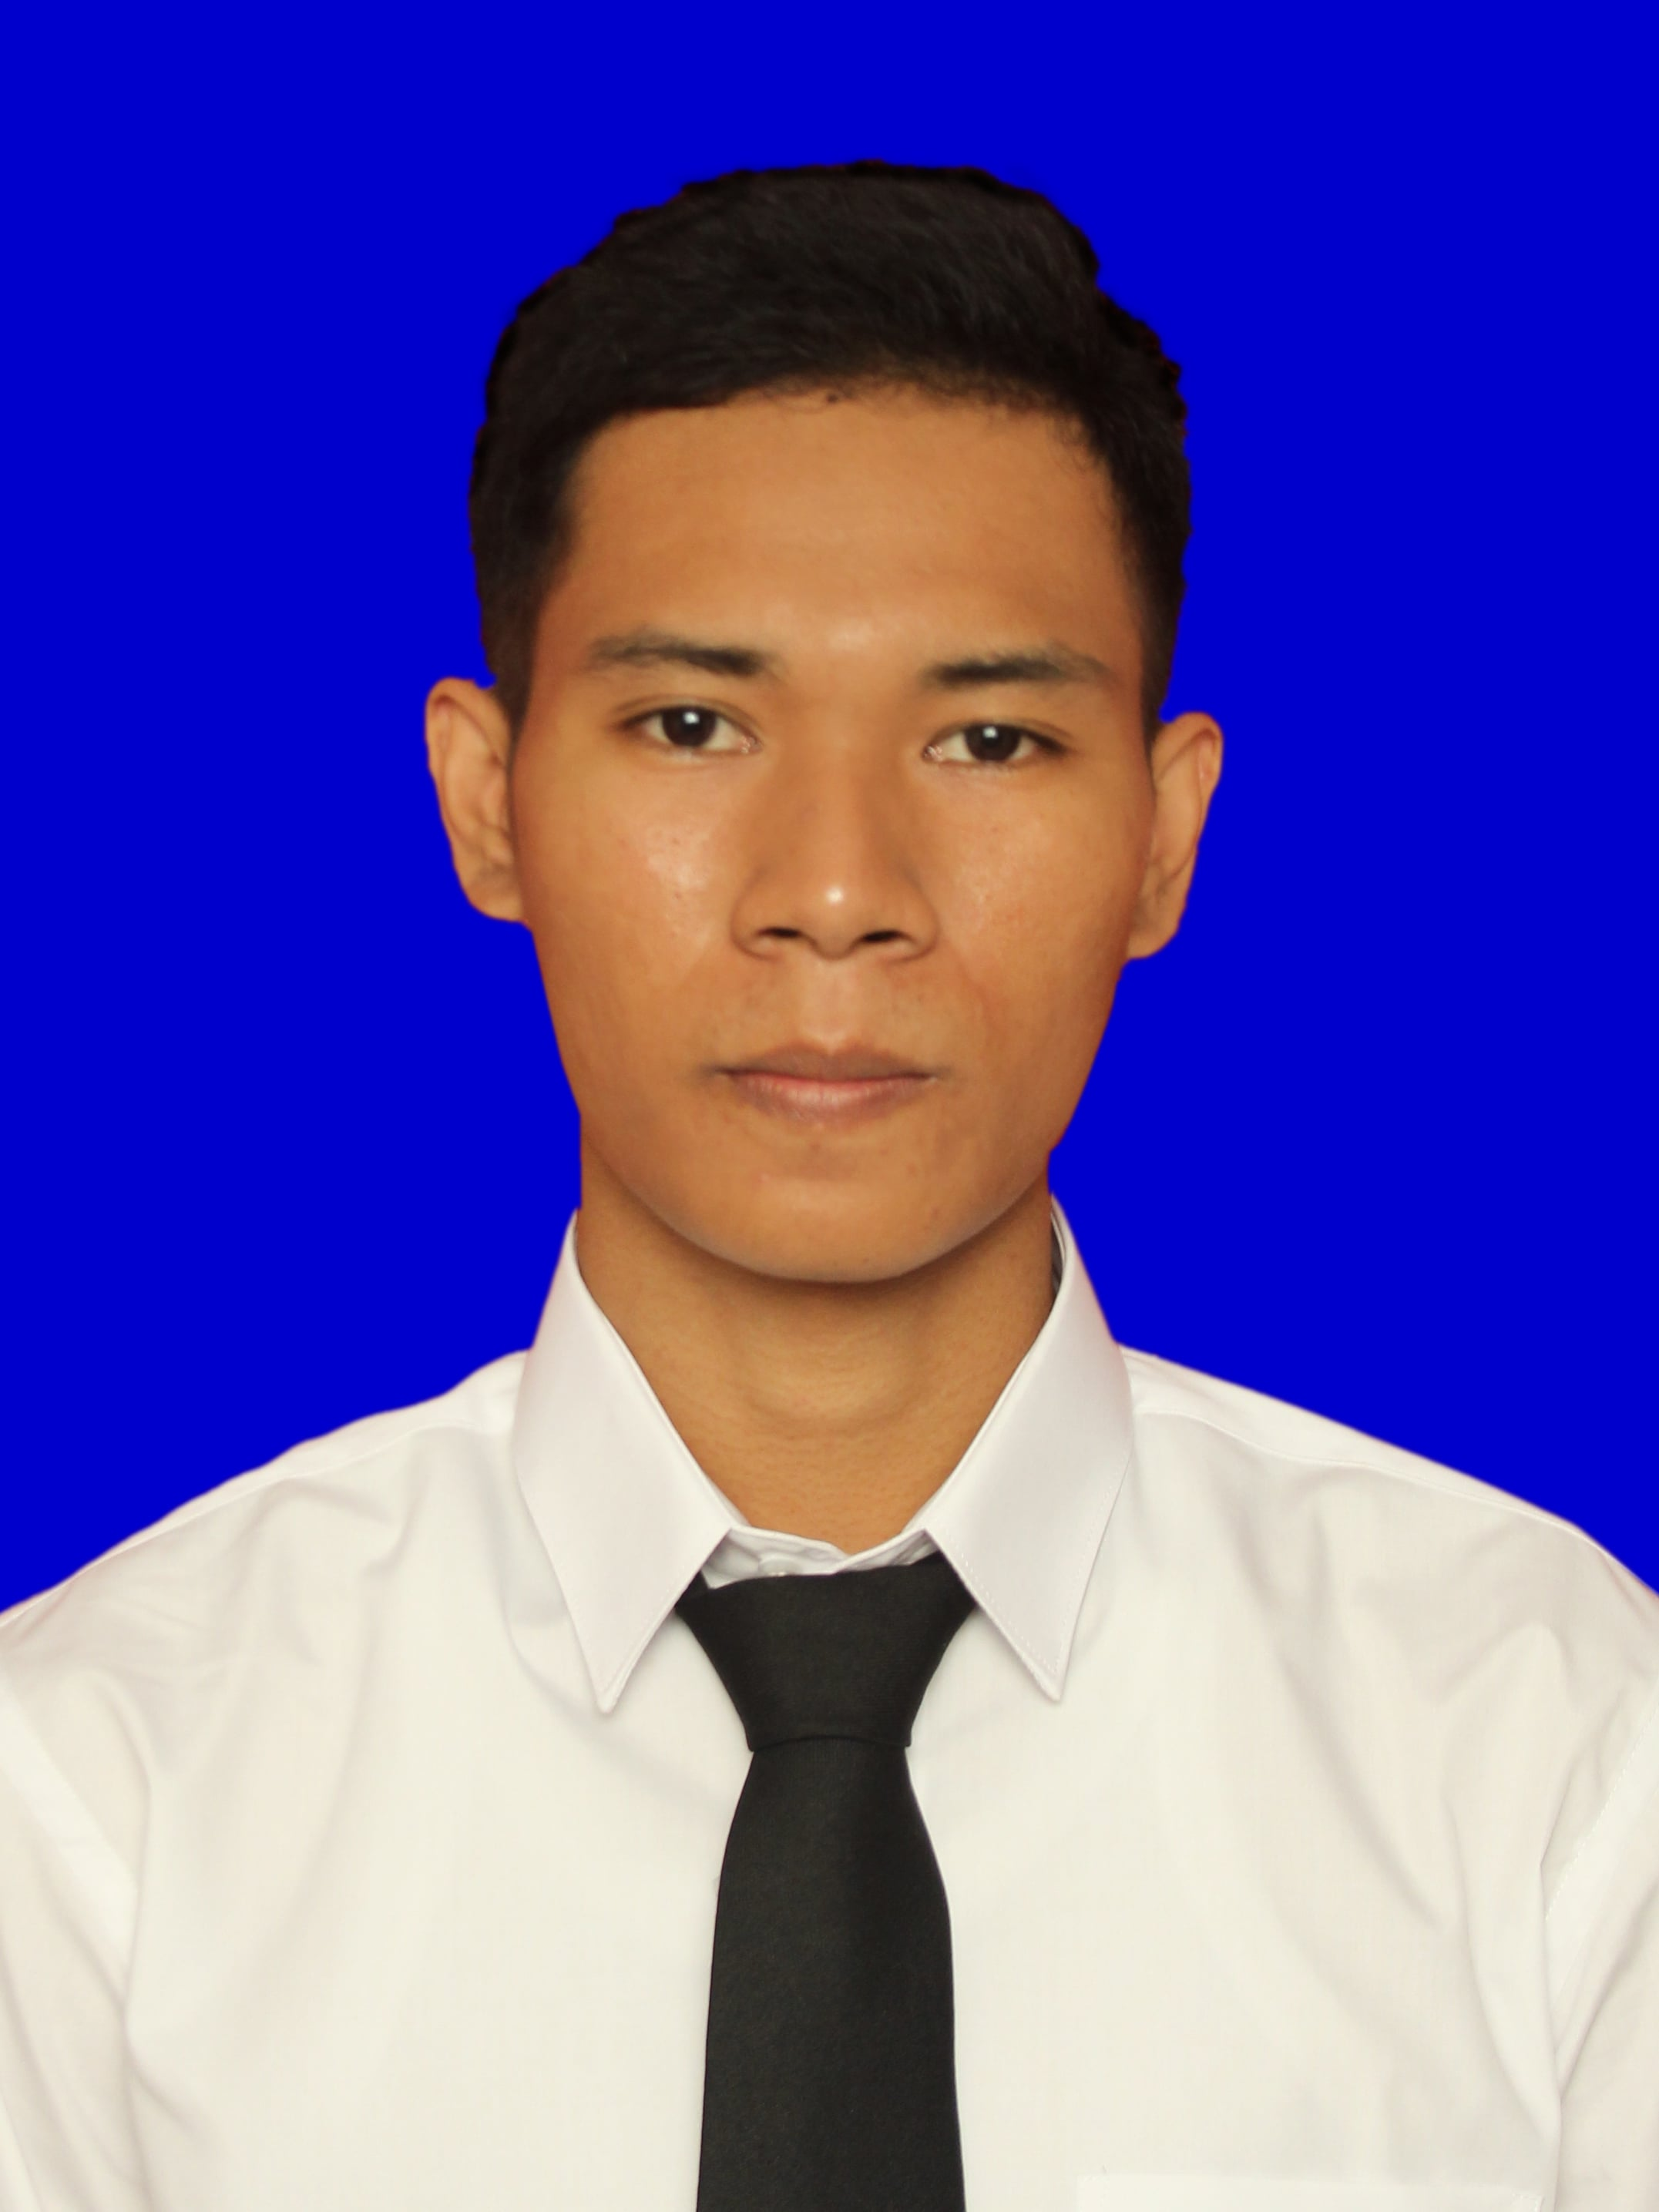
\includegraphics[width=0.3\textwidth]{gambar/HarisSetiadi.jpg}
  \vspace{-4ex}
\end{wrapfigure}

% Ubah kalimat berikut dengan biografi dari mahasiswa
\name{}, atau yang biasa dikenal dengan Haris, lahir pada tanggal 21 Maret 2000 di kota Denpasar. Penulis merupakan anak pertama dari tiga bersaudara yang tinggal dan besar di Denpasar, Bali. Setelah lulus dari SMA Negeri 2 Denpasar, penulis kemudian melanjutkan pendidikan ke jenjang strata satu di Departemen Teknik Komputer, Fakultas Teknologi Elektro dan Informatika Cerdas, Institut Teknologi Sepuluh Nopember mulai tahun 2019. 

Penulis merupakan orang yang aktif berorganisasi, dan memiliki berbagai \emph{softskill} serta \emph{hardskill}. Hal ini dibuktikan dengan rekam jejak organisasi dan kepanitiaan dari penulis seperti, Wakil Kepala Departemen Pengabdian Masyarakat Tim Pembina Kerohanian Hindu (TPKH-ITS), Wakil Ketua Internal pada TPKH Festival 2021, Staff Generasi Baru Indonesia (GenBI ITS), Staff Himpunan Mahasiswa Teknik Komputer (HIMATEKKOM ITS), hingga menjadi \emph{Product Manager} salah satu kelompok pada Bootcamp MyDigitalAcademy yang diselenggarakan oleh Bank Mandiri.